\documentclass[portrait]{sciposter}

\usepackage{a0size}
\usepackage{amsmath}
\usepackage{amssymb}
\usepackage{multicol}
\usepackage[english]{babel}
\usepackage{setspace}
\usepackage[pdftex,final]{graphicx}  % graphics (PDFTeX)
\usepackage{epsfig}
\usepackage{dsfont}
\usepackage{bm}
\usepackage{pstricks,pst-grad}
\usepackage{color}
\usepackage[square,numbers]{natbib}

\usepackage{amscd}
%\usepackage{subfigure}

%\def\ManuPath{./}

%this makes the \clines more thick
\newlength{\arrayrulewidthOriginal}
\newcommand{\Cline}[2]{%
  \noalign{\global\setlength{\arrayrulewidthOriginal}{\arrayrulewidth}}%
  \noalign{\global\setlength{\arrayrulewidth}{#1}}\cline{#2}%
  \noalign{\global\setlength{\arrayrulewidth}{\arrayrulewidthOriginal}}}

%\definecolor{BoxCol}{rgb}{0.9,0.9,0.9}
% uncomment for grey background to \section boxes 
% for use with default option boxedsections
\definecolor{BoxCol}{rgb}{0.1,0.1,0.8}
\definecolor{TextColTitle}{rgb}{0.1,0.1,0.8}

\definecolor{SectionCol}{rgb}{1,1,1}
% uncomment for dark blue \section text 
\definecolor{TextColG}{rgb}{0.1,0.0,0.8}
\definecolor{TextColR}{rgb}{0.9,0,0}
\newcommand{\Rcolor}{\textcolor{TextColR}}
\newcommand{\Gcolor}{\textcolor{TextColG}}

\setlength{\parindent}{0pt}
\setlength{\parskip}{1ex plus 0.5ex minus 0.2ex}

%-------------------------------------------------------------------------------------------------------
\title{{\Huge Hierarchically Supervised Latent Dirichlet Allocation}}

\author{
Adler Perotte\hspace{1cm} Nicholas Bartlett \hspace{1cm} No\'emie Elhadad \hspace{1cm} Frank Wood\\
Columbia University, New York, NY 10027, USA \\
%\texttt{\{ajp9009@dbmi,bartlett@stat,noemie@dbmi,fwood@stat\}.columbia.edu}
%\texttt{pfau@neurotheory.columbia.edu} 
%\texttt{\{bartlett,fwood\}@stat.columbia.edu} 
}


%\author{D.J. Albers \hspace{2 in} Noemie Elhadad \hspace{2in} George
%  Hripcsak  \hspace{2in} Esteban Tabuk}

%\institute{Columbia University \hspace{2.0 in} Columbia University
%  \hspace{2.0 in} Columbia University \hspace{2.0 in} Courant Institute (NYU)}

%\email{\hspace{1 in}\{pdeleon,vijendra\}@nmsu.edu\hspace{5 in} pucher@ftw.at\hspace{3 in} jyamagis@inf.ed.ac.uk\hspace{0 in}}

% The following commands can be used to alter the default logo settings
%\leftlogo[1.0]{Figures/NMlogo}  % defines logo to left of title (with scale factor)
\rightlogo[1]{crown2}  % same but on right

%-------------------------------------------------------------------------------------------------------
\begin{document}

%define conference poster is presented at (appears as footer)
%\conference{NIPS 2011}

\maketitle
\begin{abstract}
\begin{center}
\parbox{70 cm}{
We introduce hierarchically supervised latent Dirichlet allocation (HSLDA), a
model for hierarchically and multiply labeled bag-of-word data.  Examples of
such data include web pages and their placement in directories, product
descriptions and associated categories from product hierarchies, and free-text
clinical records and their assigned diagnosis codes. Out-of-sample label
prediction is the primary goal of this work, but improved lower-dimensional
representations of the bag-of-word data are also of interest. We demonstrate HSLDA on large-scale data from clinical document labeling and
retail product categorization tasks. We show that leveraging the structure from
hierarchical labels improves out-of-sample label prediction substantially when
compared to models that do not. 
}
\end{center}
\end{abstract}

%%% Begin of Multicols-Enviroment
\begin{multicols}{3}

%-------------------------------------------------------------------------------------------------------
\section{\textsc{Introduction}}

\begin{itemize}
\item Our work operates within the framework of topic modeling. 
\item Our approach learns
topic models of the underlying data and labeling strategies in a joint model,
while leveraging the hierarchical structure of the labels. 
\item For the sake of
simplicity, we focus on is-a hierarchies, but the model can be
applied to other structured label spaces. 
\item Our work extends supervised latent Dirichlet
allocation (sLDA)~\citep{BleiMcAuliffe2008} to take advantage of hierarchical
supervision and proposes an efficient way to incorporate such information into the model. 
\item We demonstrate our model on large, real-world datasets in the clinical and web
retail domains.
\end{itemize}
%We hypothesize that the context of labels within
%the hierarchy provides valuable information about labeling. Other models, such as LabeledLDA~\citep{Ramage2009}, incorporate LDA and supervision; however, none of these models leverage dependency structure in the label space.


%We observe that hierarchical information is valuable when
%incorporated into the learning and improves our primary goal of multi-label
%classification. Our results show that a joint, hierarchical model outperforms a
%classification with unstructured labels as well as a disjoint model, where the
%topic model and the hierarchical classification are inferred
%independently of each other. 


%\begin{figure}
%\centering
%\includegraphics[width=18cm]{final_dry.pdf}
%\small{\caption{Dry geostrophic adjustment}}
%\end{figure}


%-------------------------------------------------------------------------------------------------------
\section{\textsc{Data}}

\subsection{Discharge Summaries and ICD-9 Codes}

\begin{figure}
\centering
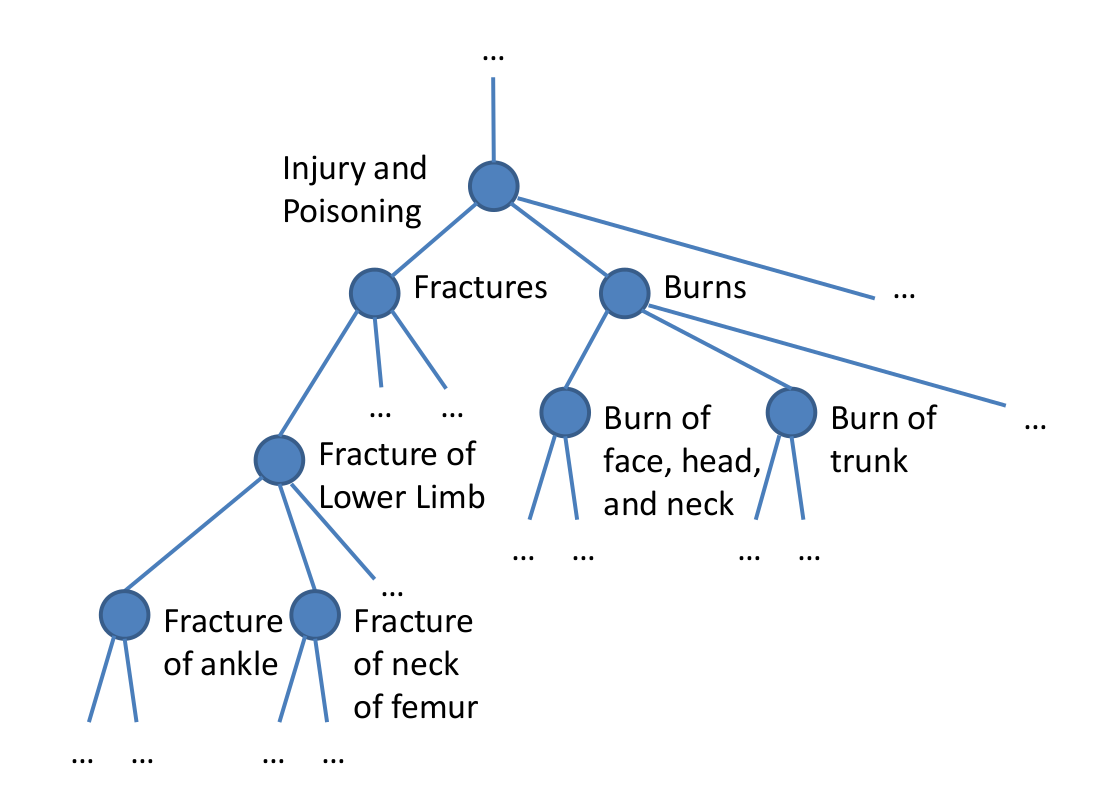
\includegraphics[width=25cm]{ICD9_crop}
\small{\caption{A Portion of the ICD9 Hierarchy}}
\end{figure}

\begin{itemize}
\item \emph{Text:} Discharge summaries are authored by clinicians to summarize patient hospitalization courses.
\begin{itemize}
\item 10000 unique words, 6000 documents, average of 536.57 terms per document (std dev=300.29)
\end{itemize}
\item \emph{Labels:} Trained medical coders review the information in the discharge summary and assign a series of diagnoses codes from a hierarcharchy called ICD9.
\begin{itemize}
\item 7298 unique codes, 6000 code sets, average of 8.39 codes per set (std dev=5.01)
\end{itemize}
\end{itemize}


\subsection{Product Descriptions and Categorizations}

\begin{figure}
\centering
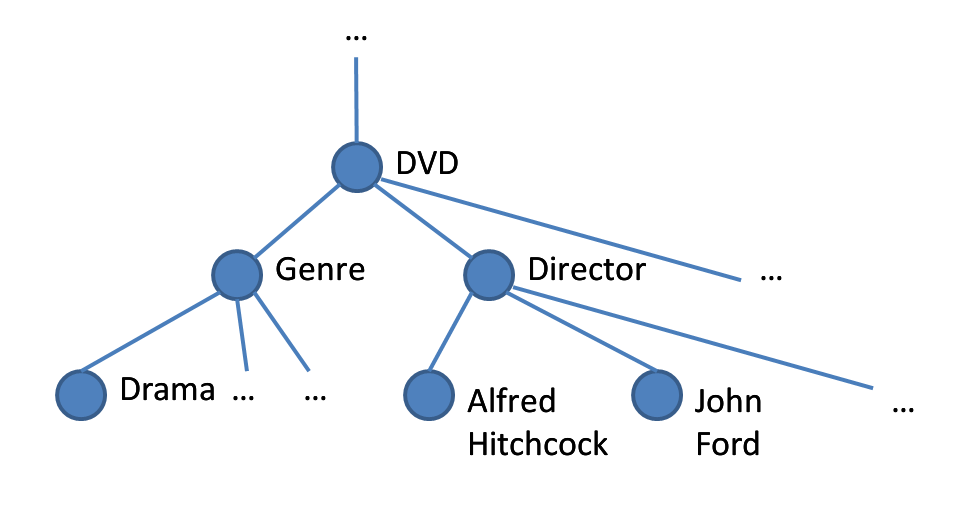
\includegraphics[width=25cm]{Amazon_crop}
\small{\caption{A Portion of the Amazon.com Hierarchy}}
\end{figure}

\begin{itemize}
\item \emph{Text:} Product descriptions were obtained from the Amazon.com website directly. We limited our dataset to the collection of DVDs in the product catalog.
\begin{itemize}
\item 30000 unique words, 16130 documents, average of 91.89 terms per document (std dev=53.08)
\end{itemize}
\item \emph{Labels:} Amazon.com product categorization data from the Stanford Network Analysis Platform (SNAP) dataset~\citep{SNAP}.
\begin{itemize}
\item 2691 unique categories, 16130 category sets, average of 9.01 codes per set (std dev=4.91) \newline \newline \newline \newline \newline \newline \newline \newline \newline
\end{itemize}
\end{itemize}


%-------------------------------------------------------------------------------------------------------
\section{\textsc{Model}}

\begin{itemize}
\item HSLDA is a model for hierarchically, multiply-labeled, bag-of-word data.

\begin{itemize}
\item Let $w_{n,d} \in \Sigma$ be the $n$th observation in the $d$th document.  
\item Let $\mathbf{w}_d = \{w_{1,d},\ldots,w_{1,N_d}\}$ be the  set of $N_d$ observations in document $d$.  
\item Let there be $D$ such documents and let the size of the vocabulary be $V=|\Sigma|$.  
\item Let the set of labels be $\mathcal{L}=\left\{  l_{1},l_{2},\ldots,l_{\left|\mathcal{L}\right|}\right\} $. 
%Each label
%$l \in \mathcal{L}$, except root, has a parent $\mathrm{pa}(l) \in \mathcal{L}$
%also in the set of labels. 
% We will for exposition purposes assume that this label set has hard ``is-a''
% parent-child constraints, although this assumption can be
% relaxed at the cost of more computationally complex inference.  Such a label hierarchy forms a multiply rooted tree.  Without loss of generality we will consider a tree with a single root $r\in\mathcal{L}$.  
\begin{itemize}
\item Each document has a variable $y_{l,d} \in \{-1,1\}$ for every label which indicates whether the label is applied to document $d$ or not.   
\item In most cases $y_{i,d}$ will be unobserved, in some cases we will be able to fix its value because of  constraints on the label hierarchy, and in the relatively minor remainder its value will be observed.  
\item In the applications we consider, only positive label applications are observed.  
\item Label responses are generated using a conditional hierarchy of probit regressors\cite{gelmanbda04}.

\end{itemize}
\end{itemize}
\end{itemize}

%In HSLDA, the bag-of-word document data is modeled using the LDA
%mixed-membership mixture model with global topic estimation.
%In HSLDA, documents are modeled using the LDA mixed-membership mixture model
%with global topic estimation. 

% The HSLDA graphical model is given in
%Figure~\ref{fig:graphical_model}. In the model, $K$ is the number of LDA
%``topics'' (distributions over the elements of $\Sigma$), $\boldsymbol\phi_k$
%is a distribution over ``words,'' $\boldsymbol\theta_d$ is a document-specific
%distribution over topics, and $\boldsymbol\beta$ is a global distribution over
%topics.


\begin{figure}
\centering
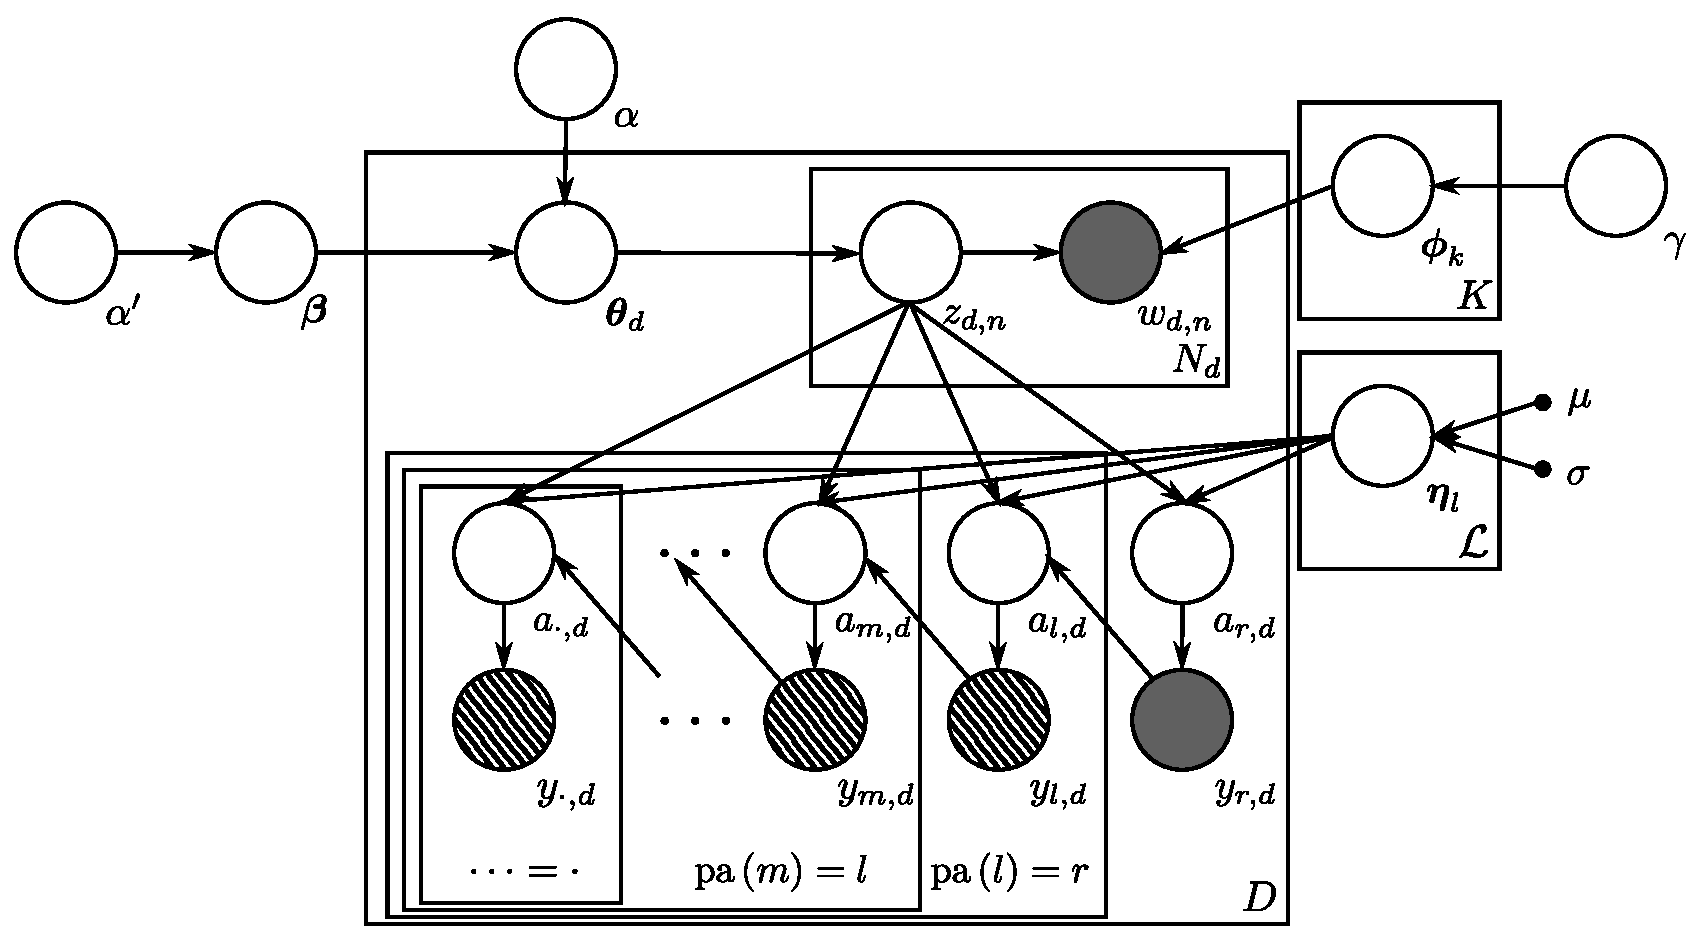
\includegraphics[width=25cm]{Graphical_Model-final}
\small{\caption{HSLDA Graphical Model}}
\label{fig:graphical_model} 
\end{figure}

\subsection{Generative Story}

%\begin{small}
\begin{enumerate}
\item For each topic $k=1,\ldots,K$

\begin{itemize}
\item Draw a distribution over words $\boldsymbol\phi_{k}\sim{\rm Dir}_{V}(\gamma\mathbf{1}_V)$%,
%where $\mathbf{1}$ is a vector of ones of length $V$ 
\end{itemize}
\item For each label $l\in\mathcal{L}$

\begin{itemize}
\item Draw a label application coefficient $\boldsymbol\eta_{l}\mid\mu,\sigma\sim\mathcal{N}_{K}(\mu \mathbf{1}_K,\sigma \mathbf{I}_{K})$  
\end{itemize}
\item Draw the global topic proportions $\boldsymbol\beta\mid\alpha'\sim{\rm Dir}_{K}\left(\alpha^{\prime}\mathbf{1}_K\right)$
\item For each document $d=1,\ldots,D$

\begin{itemize}
\item Draw topic proportions $\boldsymbol\theta_d\mid\boldsymbol\beta,\alpha\sim{\rm Dir}_{K}\left(\alpha\boldsymbol\beta\right)$ 
\item For $n=1,\ldots,N_{d}$

\begin{itemize}
\item Draw topic assignment $z_{n,d}\mid\boldsymbol\theta_d\sim{\rm Multinomial}(\boldsymbol\theta_d)$ 
\item Draw word $w_{n,d}\mid z_{n,d},\boldsymbol\phi_{1:K}\sim{\rm Multinomial}(\boldsymbol\phi_{z_{n,d}})$ 
\end{itemize}
\item Set $y_{r,d} = 1$
\item For each label $l$ in a breadth first traversal of $\mathcal{L}$ starting at the children of  root $r$

\begin{itemize}
\item Draw $a_{l,d}\mid \bar{\mathbf{z}}_d,\boldsymbol\eta_{l},y_{\mathrm{pa}(l),d}\sim\begin{cases}
\mathcal{N}(\bar{\mathbf{z}}^{T}_d\boldsymbol\eta_{l},1), & y_{\mathrm{pa}(l),d}=1\\
\mathcal{N}(\bar{\mathbf{z}}^{T}_d\boldsymbol\eta_{l},1)\mathbb{I}(a_{l,d}<0), & y_{\mathrm{pa}(l),d}=-1\end{cases}$ %\item Draw $a_{l, d} \ | \ z_{1:N_d,d}, \boldsymbol\beta_l \sim \mathcal{N} \left(\bar z_d^{T} \boldsymbol\beta_{l},1\right)$, where $\bar z_d=N_d^{-1}\sum_{n=1}^{N_d}z_{n,d}$ 
 
\item Apply label $l$ to document $d$ according to $a_{l,d}$ \[\hspace{-2cm}
y_{l,d}\mid a_{l,d}=\begin{cases}
\ \ \ 1 & \text{if \ensuremath{a_{l,d}>0}} \\% and \ensuremath{y_{{\rm \mathrm{pa}}(l),d}=1}}\\
-1 & \text{otherwise}\end{cases}\]
 
\end{itemize}
\end{itemize}
\end{enumerate}
%\end{small}
%--------------------------------------------------------------------------------------------------------

\section{\textsc{Inference}}

We define a collapsed Gibbs sampler for HSLDA where the topic assignments are sampled according to:  
%We have analytically marginalized out the parameters $\boldsymbol{\phi}_{1:K}$
%and $\boldsymbol{\theta}_{1:D}$  in the following expressions.   Let $\mathbf{a}$ be the set of all auxiliary variables, $\mathbf{w}$  the set of all words, $\boldsymbol\eta$  the set of all regression coef%ficients, and  $\mathbf{z}_d\backslash z_{n,d}$  the set $\mathbf{z}_d$ with element $z_{n,d}$ removed.  The conditional posterior distribution of the latent topic indicators is
\begin{eqnarray*}
\lefteqn{p\left(z_{n,d}=k\mid\mathbf{z}_d\backslash z_{n,d},\mathbf{a},\mathbf{w},\mathbf{\boldsymbol\eta},\alpha,\boldsymbol\beta,\gamma\right)\propto}\nonumber \\
 & \hspace{2cm}\left(c_{\left(\cdot\right),d}^{k,-\left(n,d\right)}+\alpha\boldsymbol\beta_{k}\right)\frac{c_{w_{n,d},\left(\cdot\right)}^{k,-\left(n,d\right)}+\gamma}{\left(c_{\left(\cdot\right),\left(\cdot\right)}^{k,-\left(n,d\right)}+V\gamma\right)}\prod_{l\in\mathcal{L}_{d}}\exp\left\{ -\frac{\left(\bar{\mathbf{z}}_{d}^{T}\boldsymbol\eta_{l}-a_{l,d}\right)^{2}}{2}\right\} \label{eq:z-likelihood}\end{eqnarray*}
% where $c_{v,d}^{k,-\left(n,d\right)}$ is the number
%of words of type $v$ in document $d$ assigned to topic $k$ omitting
%the $n$th word of document $d$. 

%The subscript $(\cdot)$'s
%indicate to sum over the range of the replaced variable, i.e.~$ {c_{w_{n,d},\left(\cdot\right)}^{k,-\left(n,d\right)}} = \sum_d {c_{w_{n,d},d}^{k,-\left(n,d\right)}}$.  Here $\mathcal{L}_{d}$ is the set of labels which are observed for document $d$.

%Given Equation \ref{eq:z-likelihood}, $p\left(z_{d,n}\mid\mathbf{z}_{-\left(d,n\right)},\mathbf{a},\mathbf{w},\mathbf{\boldsymbol\eta},\alpha,\boldsymbol\beta,\gamma\right)$
%can be sampled through enumeration. 

%The conditional posterior distribution of the regression coefficients is given by 
The regression coefficients are sampled according to:
\begin{equation*}
p(\boldsymbol\eta_{l}\mid\mathbf{z},\mathbf{a},\sigma) = \mathcal{N}(\hat{\boldsymbol\mu}_{l},\hat{\mathbf{\Sigma}})\label{eqn:regression_param_conditional}
\end{equation*}
%$\boldsymbol\eta_{l}$ for $l\in\mathcal{L}$. Given that $\boldsymbol\eta_{l}$
%and $a_{l,d}$ are distributed normally, the posterior distribution
%of $\boldsymbol\eta_{l}$ is normally distributed with mean $\hat{\boldsymbol\mu}_{l}$
%and covariance $\hat{\mathbf{\Sigma}}$ such that % (probably not the right place for this) We evaluated the model over various values of $\sigma$ where $\sigma=\left\{ 0.01,0.1,0.25,1,2\right\} $.
where
\begin{equation*}
\hat{\boldsymbol\mu}_{l}  =  \hat{\mathbf{\Sigma}}\left(\mathbf{1}\frac{\mu}{\sigma}+\bar{\mathbf{Z}}^{T}\mathbf{a}_{l}\right) \qquad \hat{\mathbf{\Sigma}}^{-1}  =  \mathbf{I}\sigma^{-1}+\bar{\mathbf{Z}}^{T}\bar{\mathbf{Z}}
.\end{equation*}
The auxiliary variables are sampled according to:
\begin{equation*}
p\left(a_{l,d,}\mid\mathbf{z},\mathbf{Y},\mathbf{\boldsymbol\eta}\right)\propto\frac{1}{\sqrt{2\pi}}\exp\left\{ -\frac{1}{2}\left(a_{l,d}-\boldsymbol\eta_{l}^{T}\mathbf{\bar{z}}_{d}\right)\right\} \mathbb{I}\left(a_{l,d}y_{l,d}>0\right).\label{eqn:a_l_d}\end{equation*}

Lastly, the document-level topic distributions are sampled according to:
\begin{equation*}
\boldsymbol\beta\mid\mathbf{z},\alpha^{\prime},\alpha\sim{\rm Dir}\left(m_{\left(\cdot\right),1}+\alpha^{\prime},m_{\left(\cdot\right),2}+\alpha^{\prime},\ldots,m_{\left(\cdot\right),K}+\alpha^{\prime}.\right)\end{equation*}
where the table counts, $m_{d,k}$, are sampled directly.



%-------------------------------------------------------------------------------------------------
\section{\textsc{Experiments}}

\begin{itemize}
\item Comparison models:
\begin{itemize}

\item sLDA with independent regressors (isolates effect of hierarchical constraints)
\item HSLDA fit by first performing LDA then fitting tree-conditional regressions (isolates effect of combined inference)
\end{itemize}
\item Parameters:
\begin{itemize}
\item Number of topics, $K$, set to 50.
\item $p\left(\alpha\right)$, $p\left(\alpha^{\prime}\right)$, and $p\left(\gamma\right)$ were gamma distributed with a shape parameter of 1 and a scale parameters of 1000. 
\end{itemize}
\end{itemize}



\subsection{Topic Examples}

%\begin{multicols}{2}
%\begin{center}
%\textbf{Clinical Topics}
%\end{center}
%\begin{center}
%\textbf{Product Topics}
%\end{center}
%\end{multicols}

\begin{small}
\begin{tabular}{|c|c||c|c|}
\hline
\multicolumn{2}{|c||}{\textbf{Clinical Topics}} &
\multicolumn{2}{|c|}{\textbf{Product Topics}} \\ \hline
MASS & WOUND & SERIES & BASEBALL \\
\hline
CANCER & FOOT & EPISODES & TEAM \\
\hline
RIGHT & CELLULITIS & SHOW & GAME \\
\hline
BREAST & ULCER & SEASON & PLAYERS \\
\hline
CHEMOTHERAPY & LEFT & EPISODE & BASKETBALL \\
\hline
METASTATIC & ERYTHEMA & FIRST & SPORT \\
\hline
LEFT & PAIN & TELEVISION & SPORTS \\
\hline
LYMPH & SWELLING & SET & NEW \\
\hline
TUMOR & SKIN & TIME & PLAYER \\
\hline
BIOPSY & RIGHT & TWO & SEASON \\
\hline
CARCINOMA & ABSCESS & SECOND & LEAGUE \\
\hline
LUNG & LEG & ONE & FOOTBALL \\
\hline
CHEMO & OSTEOMYELITIS & CHARACTERS & STARS \\
\hline
ADENOCARCINOMA & TOE & DISC & FANS \\
\hline
NODE & DRAINAGE & GUEST & FIELD \\
\hline
\end{tabular}
\end{small}


\subsection{Prediction}

\begin{figure}
\centering
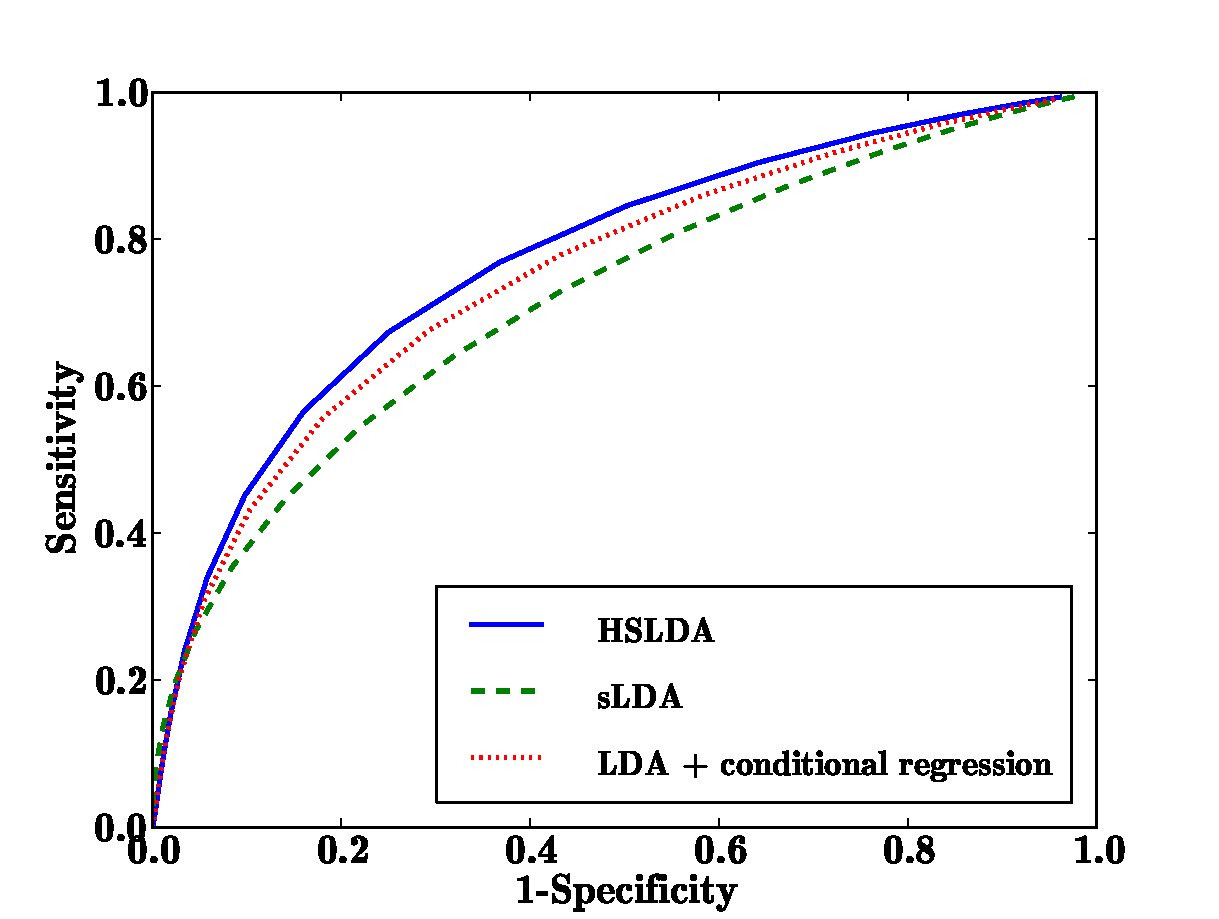
\includegraphics[width=25cm]{ROC_comparison_leafs}
\small{\caption{ROC curve for held-out ICD9 prediction varying auxiliary variable threshold.}}
\label{ICD9_aux_results}
\end{figure}

\begin{multicols}{2}

\begin{figure}
\centering
\includegraphics[width=11cm]{clin_pred_varying_mu}
\small{\caption{ROC curve for held-out ICD9 prediction varying regression parameter regularization.}}
\label{ICD9_mu_results}
\end{figure}


\begin{figure}
\centering
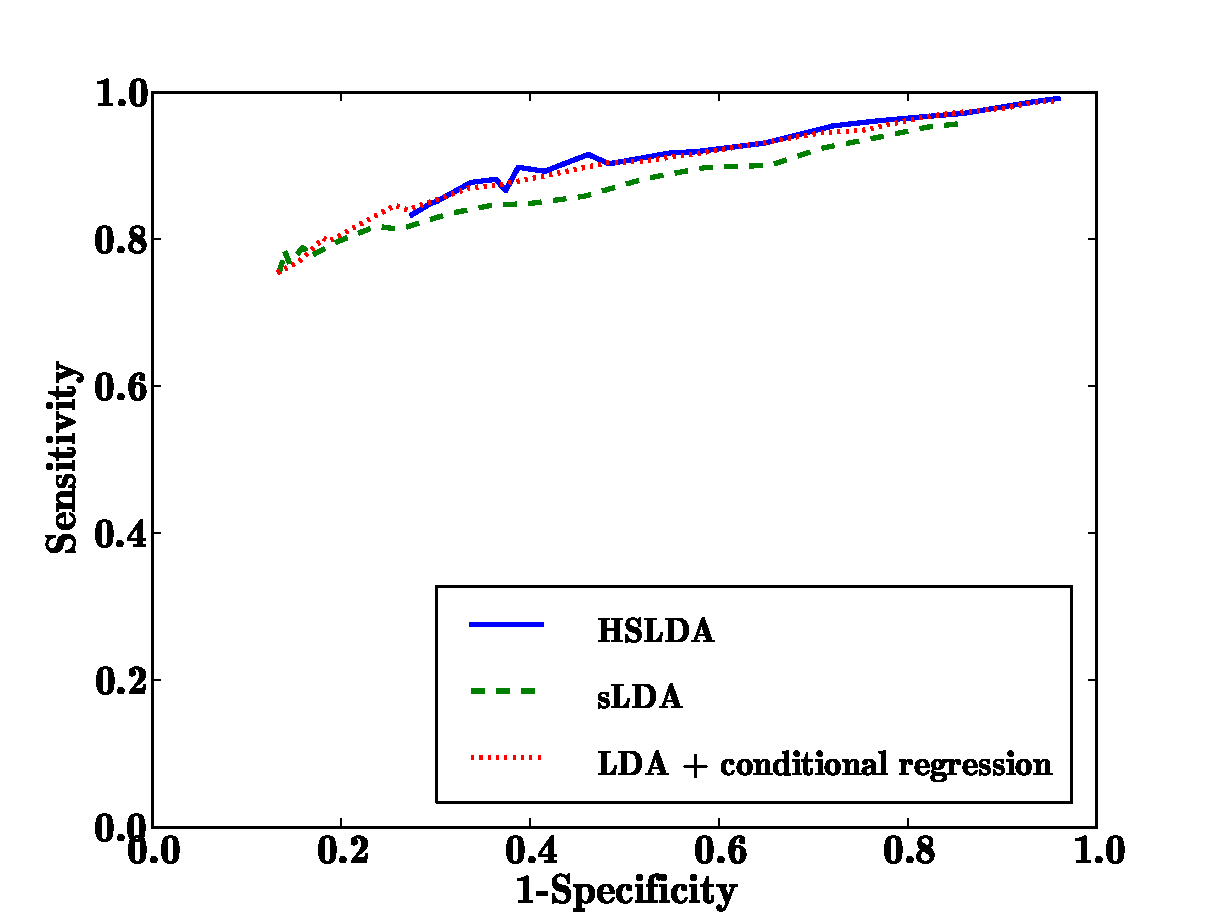
\includegraphics[width=11cm]{amazon_pred_varying_mu}
\small{\caption{ROC curve for held-out product categorization prediciton varying regression parameter regularization.}}
\label{Amazon_mu_results}
\end{figure}

\end{multicols}

%\begin{figure}[h]
%\begin{center}
%\subfigure[][]{\label{fig:1a}\includegraphics[width=.3\textwidth]{clin_pred_varying_mu}}
%\subfigure[][]{\label{fig:1b}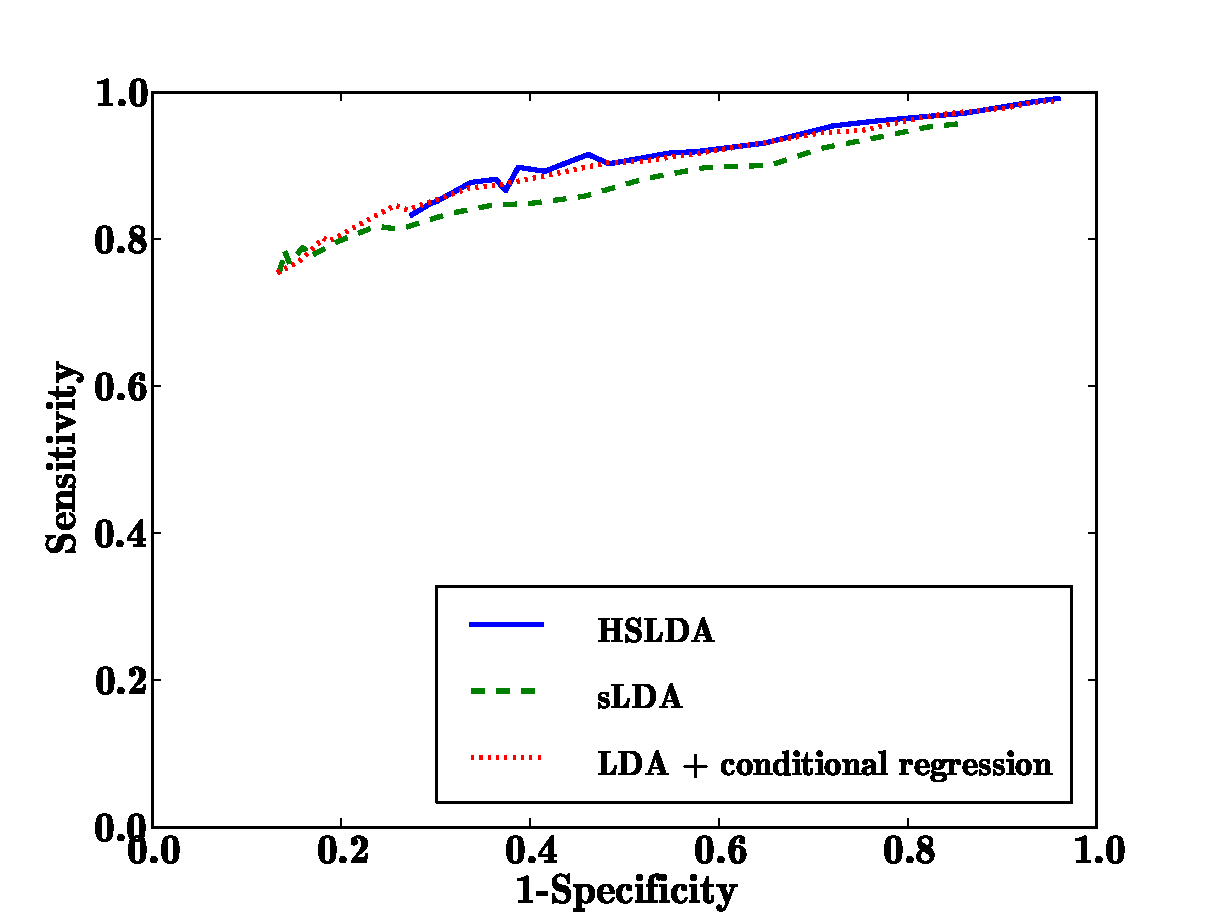
\includegraphics[width=.3\textwidth]{amazon_pred_varying_mu}}
%\subfigure[][]{\label{fig:clinical_roc}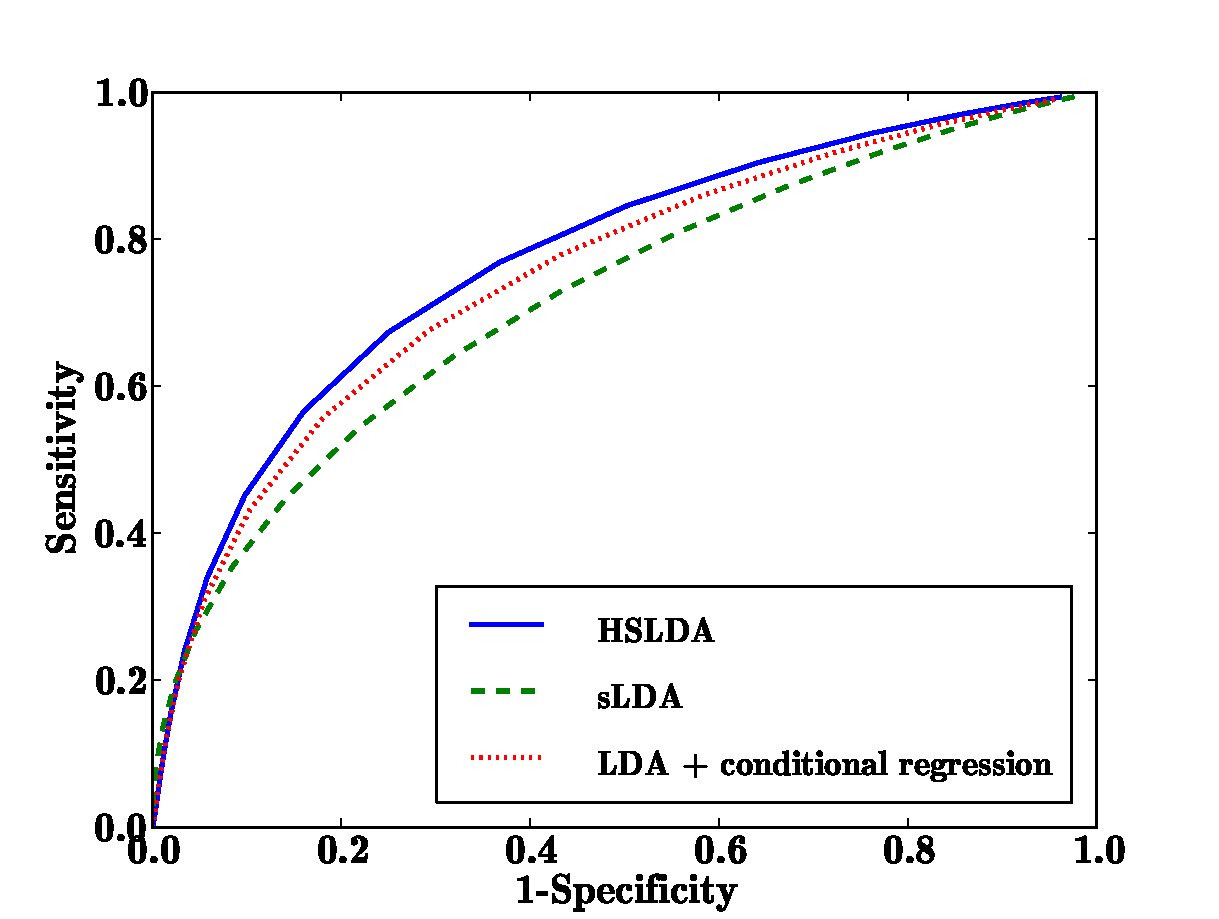
\includegraphics[width=0.3\textwidth]{ROC_comparison_leafs}}
%\caption{ROC curves for out-of-sample ICD-9 code prediction from patient free-text discharge records 
%(\subref{fig:1a},\subref{fig:clinical_roc}). ROC curve for out-of-sample Amazon product category predictions from 
%product free-text descriptions \subref{fig:1b}. Figures \subref{fig:1a} and \subref{fig:1b} are a function 
%of the prior means of the regression parameters. Figure \subref{fig:clinical_roc} is a function of auxiliary variable threshold. In all figures, solid is 
%HSLDA, dashed are independent regressors + sLDA (hierarchical 
%constraints on labels ignored), and dotted is HSLDA fit by running LDA first then running 
%tree-conditional regressions.}
%\label{fig:main_results}
%\end{center}
%\end{figure}

%-------------------------------------------------------------------------------------------------
\section{\textsc{Conclusions}}

\begin{itemize}
\item We present an efficient Gibbs sampler for sLDA based models.
\item The results in Figures~\ref{ICD9_aux_results}, \ref{ICD9_mu_results} and \ref{Amazon_mu_results} suggest that in most cases it is better to do full joint estimation of HSLDA when the label space is strongly structured.
\item One can, in an engineering sense, get nearly as much gain in label prediction performance by first fitting LDA and then fitting a hierarchical probit regression.  There are applied settings in which this could be advantageous.
\end{itemize}



% References

\begin{small} \bibliographystyle{plainnat} \bibliographystyle{plainnat}
\bibliographystyle{plainnat}
\bibliography{refs}

\end{small}

\end{multicols}

\end{document}



